\subsection{Ligne de mise à feu}
\label{subsec:ligne_mise_a_feu}

La ligne de mise à feu est conçue pour assurer l'allumage fiable et sécurisé du moteur de la fusée SP-02. Elle comprend
deux optocoupleurs servant à isulé chaque partie de la ligne de mise à feu, ainsi qu'un système de sécurité "shunt" pour éviter
tout allumage accidentel.\\

\begin{figure}[h!]
    \centering
    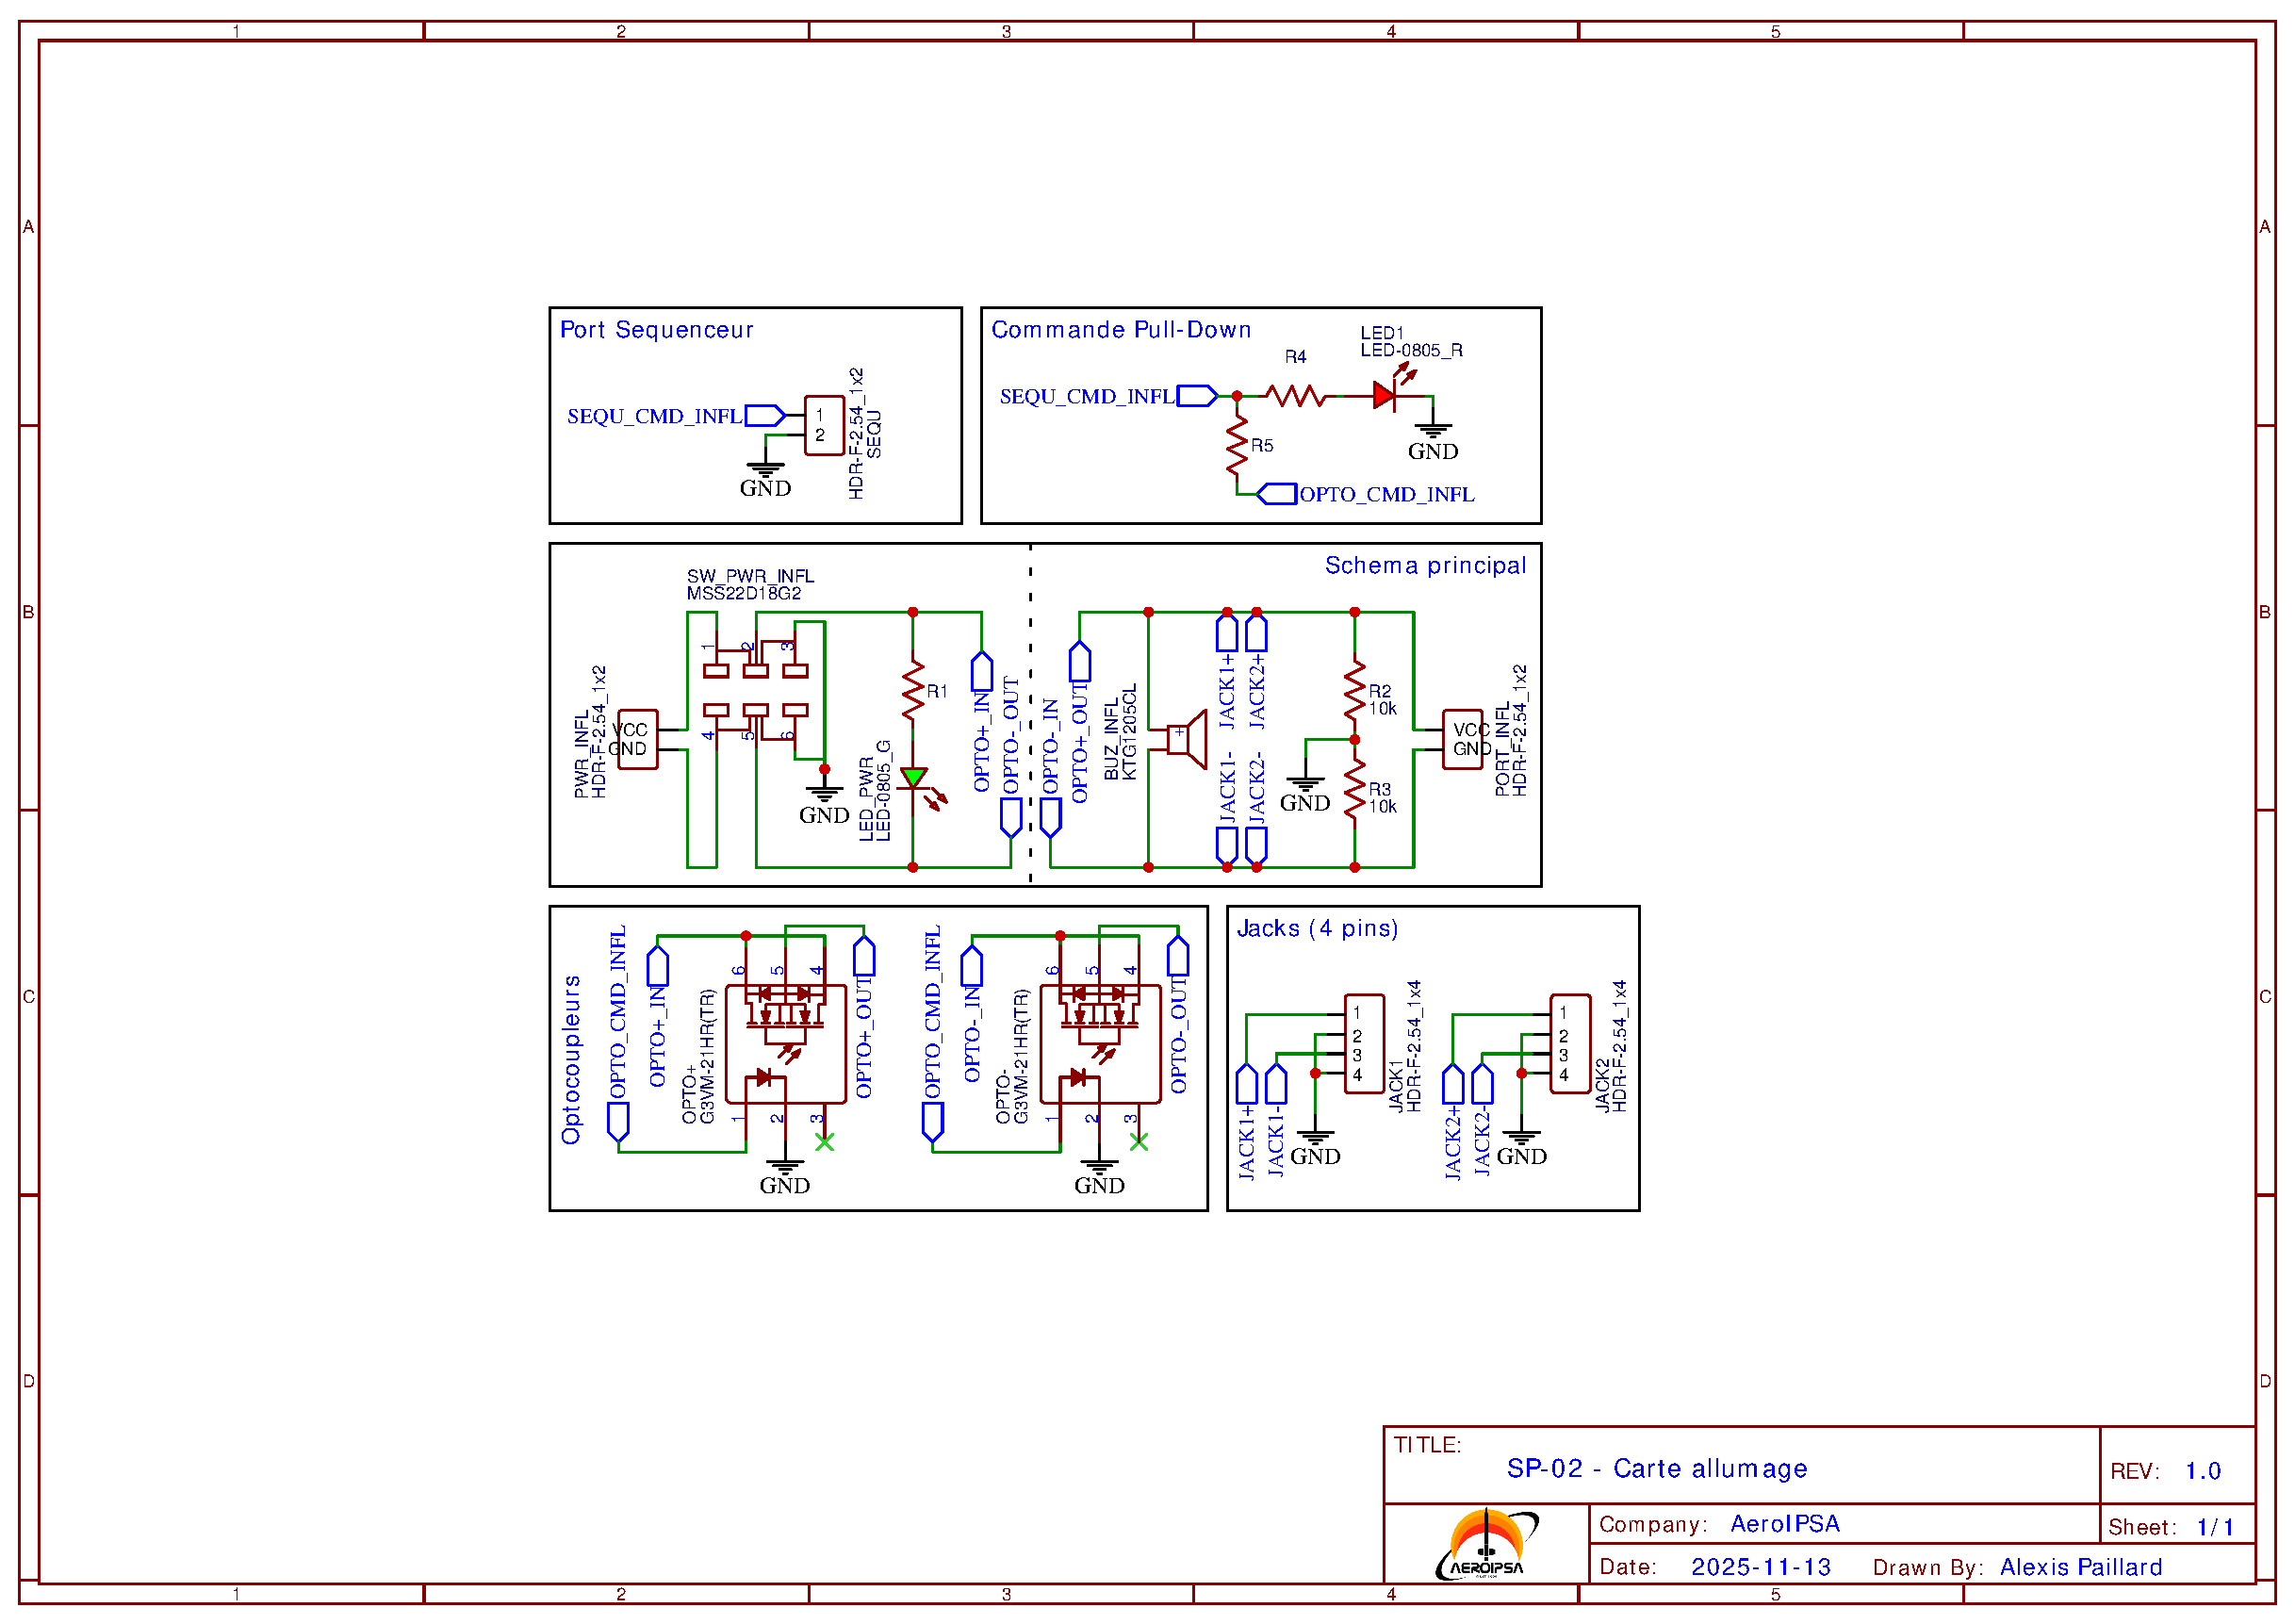
\includegraphics[width=\textwidth]{figures/Schematic_SP02_Allumage_2025-11-30.pdf}
    \caption{Schéma électrique de la ligne de mise à feu}
    \label{fig:schema_ligne_mise_a_feu}
\end{figure}

\newpage
